\documentclass[9pt]{beamer}
\mode<presentation>

  \usetheme{Szeged}

	\usecolortheme{beaver}
%\setbeamertemplate{navigation symbols}{}

	%\beamersetuncovermixins{\opaqueness<1>{25}}{\opaqueness<2->{15}}
\usepackage[francais]{babel}
\usepackage[utf8]{inputenc}
%\usepackage[T1]{fontenc}
\usepackage[lined,boxed,commentsnumbered,french,onelanguage]{algorithm2e}

\AtBeginSubsection[]{
	\begin{frame}<beamer>
		\frametitle{Plan}
		\tableofcontents[currentsection,currentsubsection]
	\end{frame}
}

\begin{document}
\title{MISE EN PLACE D'UN OUTIL DE MARQUAGE DE DOCUMENTS HTML}  
\author{Réalisé par : BOHOUSSOU Yao Yann Vianney  \& ABDOU MALAM Idriss }
%\date{Lundi, le 29 juin 2015} 


\frame{
		\begin{minipage}[t]{0.48\textwidth}
				\begin{flushleft}
					
\includegraphics{ensiasLogo.jpg} \\
				\end{flushleft}
			\end{minipage}
			
	\begin{center}
		SOUTENANCE DE PROJET INGENIERIE DU WEB \\
	\end{center}
	\titlepage
}

\frame{
	\frametitle{PLAN}
	\tableofcontents
} 

\section{Architecture globale de l'application}
\frame{
	\frametitle{Architecture globale de l'application}
		\begin{flushleft}
			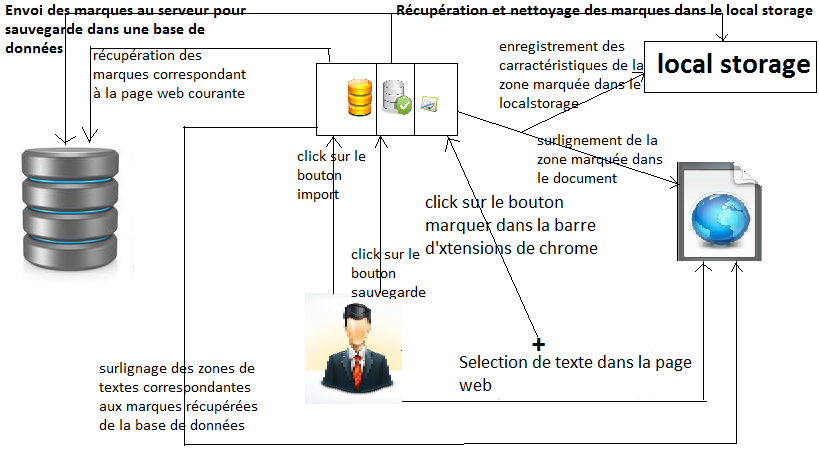
\includegraphics[width=110mm]{archiGlob.png}
		\end{flushleft}
}

\section{Traitements}
\frame
{
	\frametitle{Traitements}
			\begin{itemize}
			\item côté client 
				\begin{itemize}
					\item Fait à l'aide de scripts 
					\item récupération des carractéristiques des marques : url,chemin dans le document,position,longueur
					\item surlignage des marques
					\item Utilisation du langage javascript, et de la technologie DOM
				\end{itemize}	
			\item côté serveur
				\begin{itemize}
					\item Fait à l'aide de page JSP et de classes java 
					\item connection à la base de données mysql.
					\item enregistrement des marques et récupération des marques sauvegardées
					\item Utilisation du langage java, du sgbd mysql, et de pages JSP
				\end{itemize}
			\item interfacage du client et du serveur à l'aide de la technologie AJAX
			\end{itemize}
}

\section{Mise en place de l'extension}
\frame
	{
		\frametitle{Mise en place de l'extension}
		\begin{itemize}
					\item création du manifest 
					\item chargement de l'extension dans le navigateur
		\end{itemize}
		
	}

\section{Démonstration}
\frame
{
	\frametitle{Démonstration}
	
}


\section{CONCLUSION}
\frame{
	\frametitle{CONCLUSION}
	\begin{itemize}
		\item outils de marquage dans un document html
		\item apport positif dasn la formation par une meilleure maitrise de javascript, AJAX et DOM.
		\item amélioration possibles :
		\begin{itemize}
			\item inclure une authentification afin de distinguer les marques éffectuées par des utilisateurs différents.
			\item marques multi-balises
			\item différentes couleurs en fonction de l'importance de la marque pour l'utilisateur. 
		\end{itemize}
		
		\item MERCI POUR VOTRE ATTENTION!
	\end{itemize} 
}

\end{document}